\subsection{User interface}\label{ssc:UIAnalysis}
% goal and target users
The goal of the user interface is to provide an overview of the assets managed by the system and enable the users to oversee them. The target users for this system are experienced in using computer programs. It is therefore not necessary to guide the user thoroughly through the system's functionalities. However, the user interface should be intuitive and should support the users in their day-to-day work tasks.
\par

% supported activities and contexts. Short bursts of usage
Setting up the system and adding all the assets and their relevant information will take time and effort on the user's part. Afterwards, however, the user will only interact with the system in short bursts when making changes. There will not be an employee assigned to the system full time, based on the fact that the main users of the system, the IT department at Aalborg Zoo, have other tasks than managing the assets. Therefore it is relevant to design the system in a way that allows the user to perform their tasks as fast as possible, and get on with their other work.
\par
Because the work periods are short, user attention is less of an issue, since the user should be able to plan their work in the system to minimize external distractions. As the users work at an IT department, it is however possible for unpredictable interruptions to occur, when other employees might come by with questions or requests. Because of this, the system should be designed in a way that allows for the users attention to be divided, at least to a certain extent, without the user making major mistakes. This can be done by making it possible to save what is being worked on before it is completely done, so the user can return to finish it later. Making the system fast and responsive can also make it easier to handle distractions, as it will be easier to quickly finish the current task, despite potential interruptions.\\

% Hvordan vil vi designe UI'et?
The user interface should only contain the most essential interface-elements. As mentioned in \autoref{ch:introduction} and \autoref{ch:problemdefinition}, the client needs an easier process for managing assets compared to existing solutions on the market. Existing solutions often present the user with a lot of fields, some irrelevant to the specific asset (see \autoref{fig:too-many-fields}). This often results in empty and unnecessary fields that are never used and just clutter the interface.

\begin{figure}[H]
    \centering
    \frame{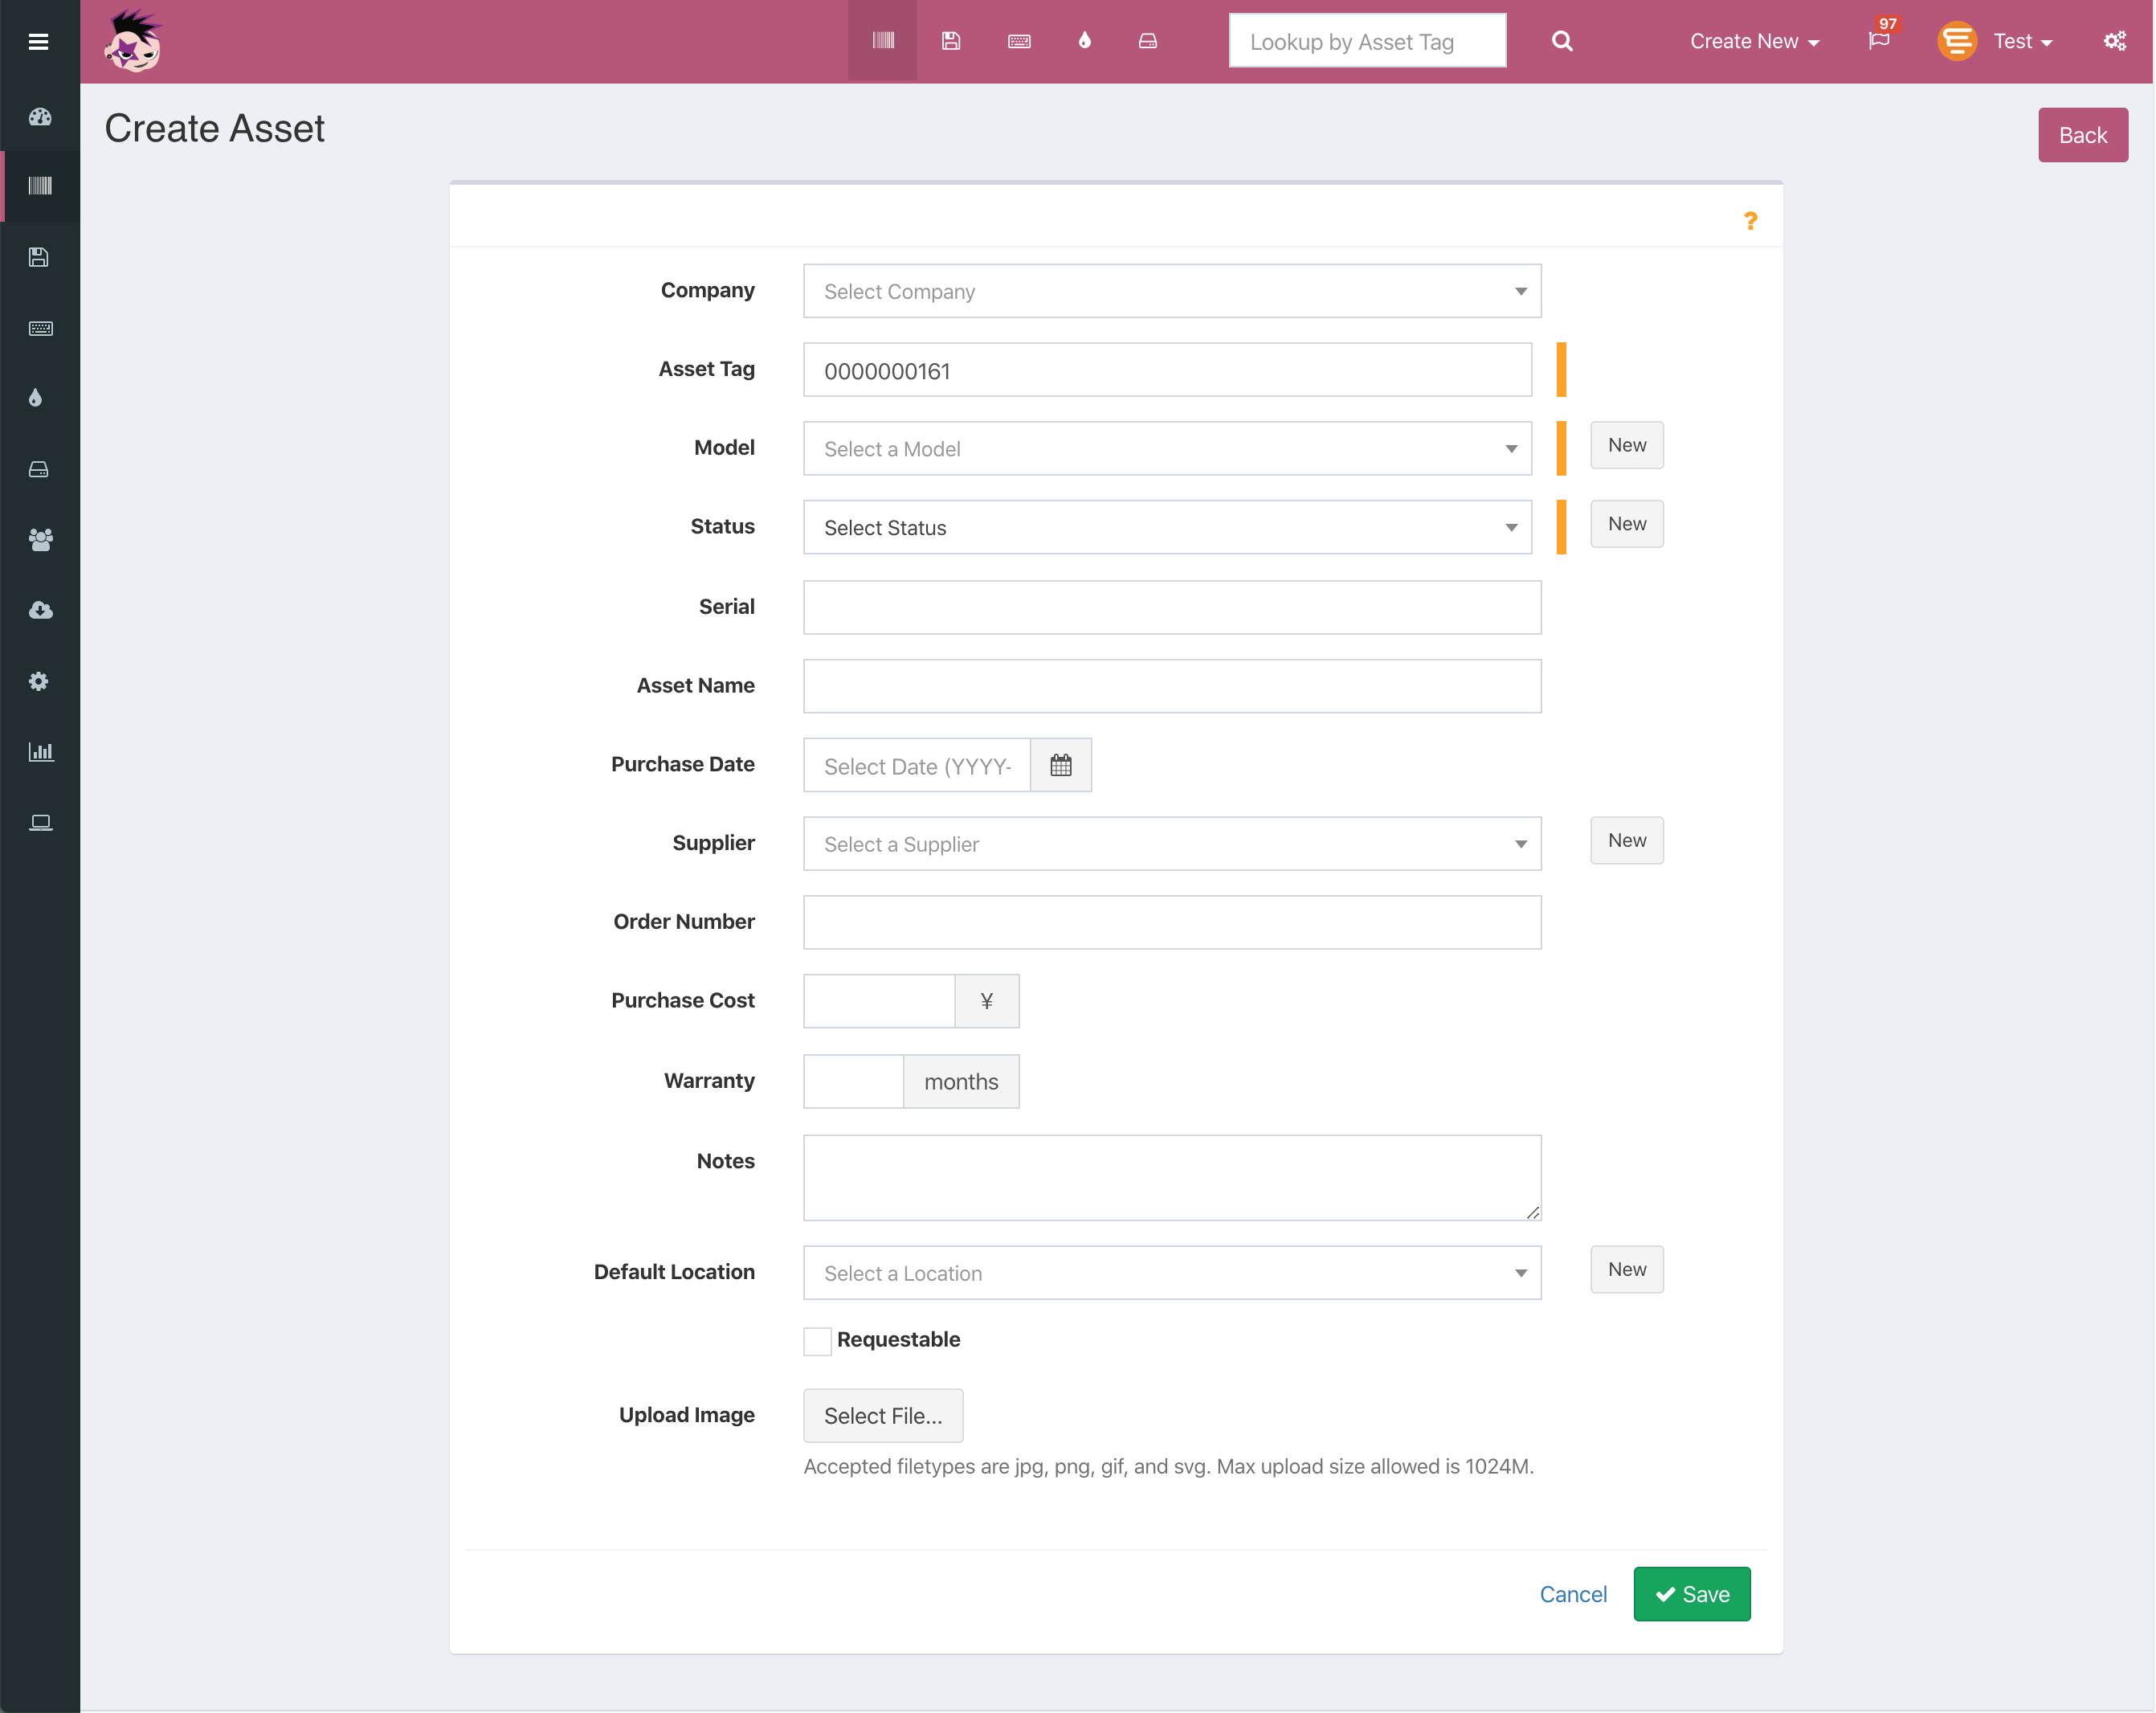
\includegraphics[width=0.9\textwidth]{figures/other-systems/snipeitapp-create-asset-ui-screenshot.png}}
    \caption{Example of an asset management system with too many fields that need to be filled out. \cite{SnipeIT}}
    \label{fig:too-many-fields}
\end{figure}

% Måske GUI vs. Command Prompt? Måske en pointe i at TUI er simplere?
Since the clients are experienced computer users, it is relevant to consider what kind of user interface the system should be implementing. A simple option is to use a text-based user interface (Terminal based User Interface, or TUI), as the employees at the IT department is expected to know how to use a terminal to access the system. The client, however, also wanted all other employees at the zoo to be able to access the system, in order to view the assets, and it is possible that other departments also will be using the system. Since it cannot be expected that employees at other departments are equally qualified to use a TUI, a graphical user interface (GUI) has been chosen instead. 
\par
Below are two pictures of ideas for a graphical user interfaces that comply with the clients wishes (see \autoref{fig:add_asset_no_tags} and \autoref{fig:add_asset_with_tags}). These pictures have been used as inspiration for the final user interface design.
\par
The pictures show how the page for adding an asset to the system looks, and how fields and tags attached to the asset could be shown.

\begin{figure}[H]
    \centering
    \frame{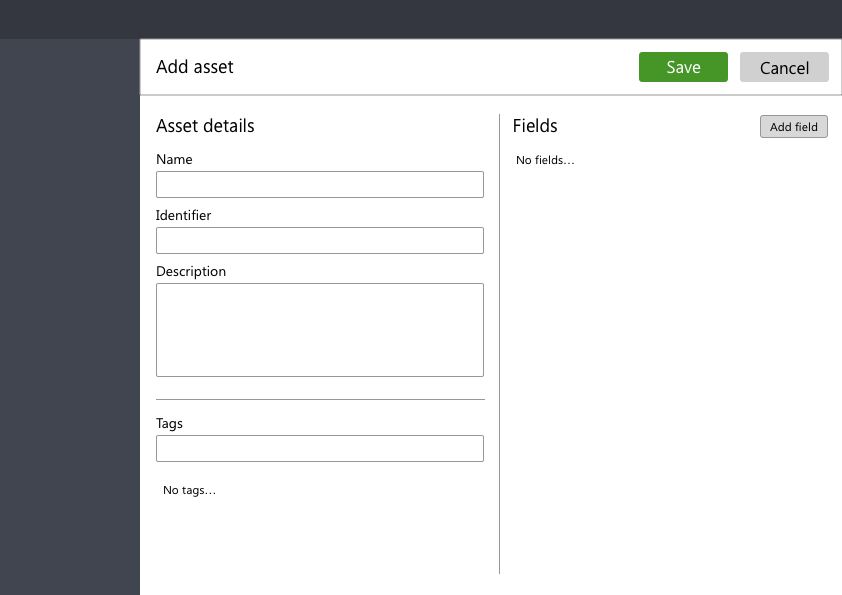
\includegraphics[width=0.9\textwidth]{figures/wireframes/add-asset-no-tags.png}}
    \caption{The process of creating a new asset. At this point no tags or custom fields have been added (right side), resulting in no fields beside the base fields (left side).}
    \label{fig:add_asset_no_tags}
\end{figure}

\begin{figure}[H]
    \centering
    \frame{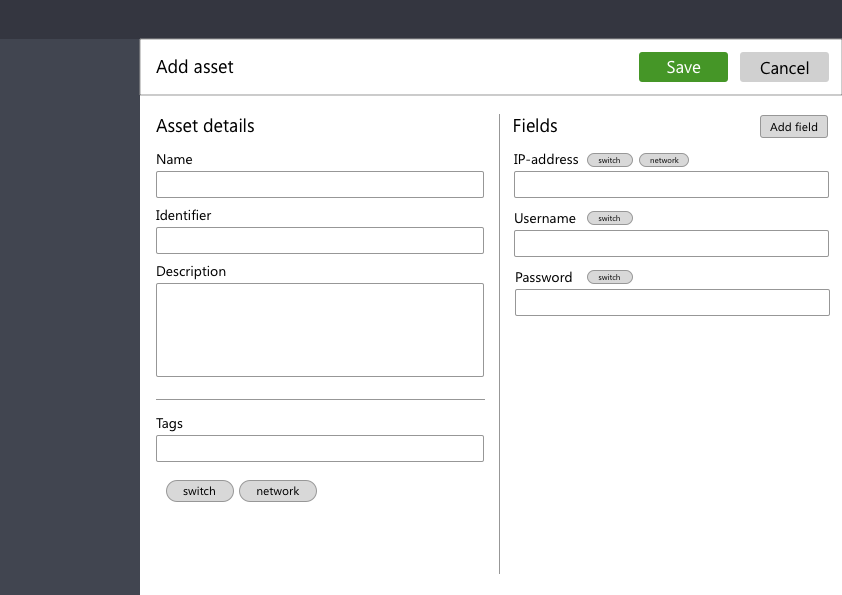
\includegraphics[width=0.9\textwidth]{figures/wireframes/add-asset-with-tags.png}}
    \caption{An example of how the user interface for adding a new asset looks after adding some tags and custom fields.}
    \label{fig:add_asset_with_tags}
\end{figure}

There are, as mentioned in previous sections, two types of users of the system, the administrators (the \textit{Admin} class) and the other employees (the \textit{Employee} class), who have much more restricted access to the system. The pictures show the user interface for the admin. If an employee user accesses the system, the interface will be limited with fewer functionalities, as these users are not allowed to make changes to the systems content.